% 请确保文件编码为utf-8,使用XeLaTex进行编译,或者通过overleaf进行编译

\documentclass[answers]{exam}  % 使用此行带有作答模块
% \documentclass{exam} % 使用此行只显示题目

\usepackage{xeCJK}
\usepackage{zhnumber}
\usepackage{graphicx}
\usepackage{hyperref}
\usepackage{amsmath}
\usepackage{amssymb}
\usepackage{mathtools}
\usepackage{booktabs}
\usepackage{enumerate}
\usepackage{enumitem} % 控制列表样式
\usepackage{listings} 

\title{2025模式识别 \\ 作业三}
\date{2025.4.15}
\pagestyle{headandfoot}
\author{人工智能学院 221300079 王俊童}
\firstpageheadrule
\firstpageheader{南京大学}{2025模式识别}{作业三}
\runningheader{南京大学}
{2025模式识别}
{作业三}
\runningheadrule
\firstpagefooter{}{第\thepage\ 页(共\numpages 页)}{}
\runningfooter{}{第\thepage\ 页(共\numpages 页)}{}

% no box for solutions
% \unframedsolutions
\def \x \mathbf{x}


\setlength\linefillheight{.5in}

% \renewcommand{\solutiontitle}{\noindent\textbf{答:}}
\renewcommand{\solutiontitle}{\noindent\textbf{解:}\par\noindent}

\renewcommand{\thequestion}{\zhnum{question}}
\renewcommand{\questionlabel}{\thequestion .}
\renewcommand{\thepartno}{\arabic{partno}}
\renewcommand{\partlabel}{\thepartno .}

\def\dist{{\mathrm{dist}}}
\def\x{{\boldsymbol{x}}}
\def\w{{\boldsymbol{w}}}


\begin{document}
% \normalsize
\maketitle
221300079 王俊童,人工智能学院
\section{问题一}
\begin{enumerate}[label=\alph*.] 
    \item 用python完成,结果如下:
    \begin{lstlisting}
        10维样本的l2范数统计:
        均值: 2.8871
        最小值: 2.0136
        最大值: 4.0669
    \end{lstlisting}
    \item 同样,用python可以得到:
    \begin{lstlisting}
        100维样本的l2范数统计:
        均值: 9.9181
        最小值: 8.8613
        最大值: 11.0844

        1000维样本的l2范数统计:
        均值: 31.7088
        最小值: 30.6157
        最大值: 32.9135

        10000维样本的l2范数统计:
        均值: 99.9484
        最小值: 98.8400
        最大值: 101.5054

        100000维样本的l2范数统计:
        均值: 316.4926
        最小值: 315.0430
        最大值: 318.7029
    \end{lstlisting}
    \item 可以提出一个猜想是:\textbf{随着维度d变高,样本的l2范数更加接近$\sqrt{d}$的取值。他们的相对波动减少}
    \par 可以理解为:\textbf{维度增加,对于d维度的标准高斯分布,l2范数越来越集中于$\sqrt{d}$附近。}
    \par 相对波动:
    \begin{equation*}
        relative\ variance = \frac{\max - \min}{mean}
    \end{equation*}
    \begin{lstlisting}
        100维样本的l2范数统计:
        波动: 0.2241

        1000维样本的l2范数统计:
        波动: 0.0725

        10000维样本的l2范数统计:
        波动: 0.0267

        100000维样本的l2范数统计:
        波动: 0.0116
    \end{lstlisting}

    \item 如果用严谨的数学语言描述这个现象,可以解释为:
    \par 令$X = (X_1, X_2, \cdots, X_d)^\top\sim \mathcal{N}(0, I_d)$,且其l2范数满足
    $\|X\|_2 = \sqrt{\sum_{i=1}^{d} X_i^2}$,其l2范数的平方服从自由度为d的$\chi^2$分布。那么有以下形式的式子在概率意义下成立:
    \begin{equation*}
        \frac{\|X\|_2}{\sqrt{d}} \xrightarrow{P} 1, \quad when\ d \rightarrow \infty
    \end{equation*}
    当然这是一个服从大数定律形式的,或者可以有一个concentration的形式:
    \begin{equation*}
        P(|\frac{\|X\|_2}{\sqrt{d}} - 1| \geq \epsilon) \rightarrow 0, \quad when\ d \rightarrow \infty
    \end{equation*}
    \item 虽然集中不等式和大数定律忘的差不多了,但是可以知道这个东西服从一定的集中不等式,或者从大数定律来解释也是可以的,最后会有一个逼近性。
\end{enumerate}

\section{问题二}
\begin{enumerate}[label=\alph*.] 
    \item 对于核函数的半正定性质,有:$y^\top K_1 y \geq 0, y^\top K_2 y \geq 0$,
    对于$K = K_1 + K_2$,有$y^\top K y = y^\top K_1 y + y^\top K_2 y \geq 0$,所以合法
    \item 同理$K = K_1 - K_2$,有$y^\top K y = y^\top K_1 y - y^\top K_2 y$,但这个不是合法的核函数,可以有一个例子是
    如果$K = 
    \begin{pmatrix}  
        -1 & 0 \\
        0 & -1 
    \end{pmatrix}$
    那么对于一个$y = (1, 0)^\top$,有$K_1 = 0, K_2 = x^\top y$,这个是不合法的,不正定。
    \item 对于$y^\top K_1y \geq 0$, 且$\alpha\geq 0$, 所以$\alpha y^\top K_1 y \geq 0$成立,所以合法。
    \item 同上$\alpha y^\top K_1 y \geq 0$成立,但是$-\alpha y^\top K_1 y \leq 0$成立,所以不合法。
    \item 对于$K = K_1 K_2$,这个是逐元素相乘,所以可以得到我们需要证明$K = K_1 K_2 \rightarrow y^\top K_1 K_2 y \geq 0$,所以我们需要证明矩阵$K_1, K_2$
    是半正定的,我们知道他们分别是半正定,所以我们可以让$K_1 = U^\top U$。所以$y^\top K_1 K_2 y  = \sum_{i=1}^{n}\sum_{j=1}^{n} y_i^\top K_1  K_2 y_j 
    = \sum_{i=1}^{n}\sum_{j=1}^{n}\sum_{k=1}^{n} (u_{ki}y_i) K_{ij} (u_{kj}y_j) \geq 0 $,所以合法.
    \item 因为$\phi$是一个合法的从d->d'的合法映射,所以对于$\{x_1, x_2, \cdots, x_n\}$,可以有$\{\phi(x_1), \phi(x_2), \cdots, \phi(x_n)\}$对于原核函数也是
    在核函数处理范围内,所以对于原来的$K = \kappa_3(\phi(x), \phi(y))$可以得到$K_3 = \kappa_3(\phi(x), \phi(y))$,$K = K_3$,由于$K_3$一定合法,所以K合法。
\end{enumerate}

\section{问题三}
\begin{enumerate}[label=\alph*.] 
    \item 因为要施加一个k,根据题目描述,可以得到k对于样本i有:
    \begin{equation*}
        k_i = \begin{cases*}
             1,\quad y_i = 1 \\
             k,\quad y_i = -1 
        \end{cases*}
    \end{equation*}
    若$f(x) = \mathbf{w}^\top \mathbf{x_i}+ b$所以优化问题变为:
    \begin{align*}
        \min_{w,b} & \frac{1}{2}\mathbf{w}^\top \mathbf{w} + C \sum_{i=1}^{n} k_i \xi_i  \\
        s.t.\quad  & y_i(\mathbf{w}^\top \mathbf{x_i} + b) \geq 1 - \xi_i, \quad 1\leq i \leq n \\
                   & \xi_i \geq 0,\quad 1\leq i \leq n
    \end{align*}
    \item 把这个问题写成lagrange形式:
    \begin{equation*}
        L = \frac{1}{2}\mathbf{w}^\top \mathbf{w} +  C \sum_{i=1}^{n} k_i \xi_i + \sum_{i=1}^{n}\alpha_i (1 - \xi_i - y_i(\mathbf{w}^\top x + b)) - \sum_{i=1}^{n}\mu_i \xi_i
    \end{equation*}
    求$\mathbf{w},b,\xi_i$的导数:
    \begin{align*}
        & \mathbf{w} = \sum_{i=1}^{n} \alpha_i y_i \mathbf{x_i}\\
        & 0 = \sum_{i=1}^{n} \alpha_i y_i \\
        & k_i C = \alpha_i + \mu_i \\
    \end{align*}
    所以带入可以得到:
    \begin{equation*}
        L = \sum_{i=1}^{n} \alpha_i - \frac{1}{2}\sum_{i=1}^{n}\sum_{j=1}^{n}\alpha_i \alpha_jy_i y_j \mathbf{x}_i^\top \mathbf{x}
    \end{equation*}
    所以对偶问题为:
    \begin{align*}
        \max_\alpha & \sum_{i=1}^{n} \alpha_i - \frac{1}{2}\sum_{i=1}^{n}\sum_{j=1}^{n}\alpha_i \alpha_jy_i y_j \mathbf{x}_i^\top \mathbf{x}\\
        s.t. \quad  & \sum_{i=1}^{n} \alpha_i y_i= 0,\quad 1\leq i\leq n,\\
                    & 0 \leq \alpha_i \leq k_i C,\quad 1\leq i\leq n,\\
    \end{align*}
    KKT条件为:
    \begin{equation*}
        \begin{cases*}
            \mu_i \geq 0, \alpha_i \geq 0\\
            (1 - \xi_i - y_i(\mathbf{w}^\top x + b)) \geq 0 \\
            \alpha_i (1 - \xi_i - y_i(\mathbf{w}^\top x + b)) = 0\\
            \xi_i \geq 0 \\
            \mu_i \xi_i = 0
        \end{cases*}
    \end{equation*}
\end{enumerate}

\section{问题四}
\begin{enumerate}[label=\alph*.] 
    \item 基本假设:属性的条件独立性假设。
    \par 优点:分类效率稳定,可以增量学习,对缺失不太敏感,可以用小数据算置信度高的结果。
    \par 缺点:条件独立性假设一般是不成立的,所以如果有关联的时候,朴素贝叶斯效果不好。
    \par 这个算法是参数化的,参数空间是有限的。
    \item 根据bayes算法,可以计算出:$P(A) = \frac{1}{3}, P(B) = \frac{1}{3}, P(C) = \frac{1}{3}.$
    \par 因为都是高斯分布,可以计算每个类别属性对应的均值和方差。
    \begin{itemize}
        \item (A,1):$\mu = 2.5, \sigma = 1.25$
        \item (A,2):$\mu = 3.5, \sigma = 1.25$
        \item (B,1):$\mu = 2.5, \sigma = 1.25$
        \item (B,2):$\mu = 5.5, \sigma = 1.25$
        \item (C,1):$\mu = 5.5, \sigma = 1.25$
        \item (C,2):$\mu = 2.5, \sigma = 1.25$
    \end{itemize}
    根据bayes,由于分母一样:
    \begin{equation*}
        P(Y_k|X) = \frac{P(XY_k)}{P(X)} = \frac{P(X|Y_k)P(Y_k)}{\sum_{j} P(X|Y_j)P(Y_j)} \sim P(X|Y_k)P(Y_k)
    \end{equation*}
    所以(只给出第一个,后面都一样):
    \begin{itemize}
        \item $P_{(x_1|A)} = 1/(\sqrt{2\pi}\sqrt{1.25})* \exp(-(2-2.5)^2/(2*1.25)) = 0.323$
        \item $P_{(x_1|B)} = 0.323$
        \item $P_{(x_1|C)} = 0.003$
        \item $P_{(x_2|A)} = 0.145$
        \item $P_{(x_2|B)} = 0.003$
        \item $P_{(x_2|C)} = 0.323$
        \item $P_{(y_1|A)} = 0.003$
        \item $P_{(y_1|B)} = 0.003$
        \item $P_{(y_1|C)} = 0.323$
        \item $P_{(y_2|A)} = 0.029$
        \item $P_{(y_2|B)} = 0.0001$
        \item $P_{(y_2|C)} = 0.145$
    \end{itemize}
    所以:
    \begin{itemize}
        \item $P(A|(x_1,x_2)) = 1/4 + 0.323 + 0.145 = 0.016$
        \item $P(B|(x_1,x_2)) = 0.00029$
        \item $P(C|(x_1,x_2)) = 0.00029$
        \item $P(A|(y_1,y_2)) = 0.0000259$
        \item $P(B|(y_1,y_2)) = 0.0000259$
        \item $P(C|(y_1,y_2)) = 0.016$
    \end{itemize}
    所以x会为A类,y会为C类。
\end{enumerate}

\section{问题五}
\begin{enumerate}[label=\alph*.] 
    \item 信息熵如下:
    \begin{align*}
        x: H &= -(0.5\log(0.5) + 0.25\log(0.25) + 0.25\log(0.25)) = 1.5\\
        y: H &= -(0.5\log(0.5) + 0.5\log(0.5)) = 1\\
        \hat{x}: H &= -(0.5\log(0.5) + 0.5\log(0.5)) = 1\\
    \end{align*}
    有损,因为在x输入是3的时候,会被还原为2.只有这种情况有损,因为信息熵减少了。

    \item D如果用MSE的话,且X是一个遵守$x\sim P(X),for i =1,\cdots, n$,y遵守$y\sim Q(Y),for j = 1,\cdots, m$, 可以表示如下:
    \begin{equation*}
        J = \frac{1}{n} \sum_{i=1}^{n} P_i\left(x_i - g(f(x_i))\right)^2 - \lambda \sum_{j=1}^{m}Q_j \log Q_j
    \end{equation*}
    对于这个式子有一个可行的优化方式是,从x到y进来不要引入损失,让码率最小,所以f=0,所以g(y)有两个取值:
    \par g(y) = 1: D = 1.25/3 = 0.4167
    \par g(y) = 2: D = 0.75/3 = 0.25
    \par 所以可以计算a中的这个系统性能如下:$J_a = 0.25/3 + \lambda$
    \par b的性能为:$J_b = 0.25$
    \par 所以
    \begin{itemize}
        \item $\lambda = 0.1$ : $J_a = 0.25/3 + 0.1 = 0.183$, $J_b = 0.25$
        \item $\lambda = 1$ : $J_a = 0.25/3 + 1 = 1.083$, $J_b = 0.25$
        \item $\lambda = 10$ : $J_a = 0.25/3 + 0.1 = 10.183$, $J_b = 0.25$
    \end{itemize}
    在0.1的时候a好,1和10的时候b好。
    \item 如果y是个两类的判别,那么输入类别只有在2类概率的时候才会无损,因为只有两类别的时候信息熵才会为1
    ,这样才能保证无损,如果是a的话,信息熵铁定大于1的,所以肯定不能保证无损。

    如果$y\in \mathbb{Z}$:
    \begin{equation*}
        J = \frac{1}{n} \sum_{i=1}^{n} P_i\left(x_i - g(f(x_i))\right)^2 - \lambda \sum_{j=1}^{\infty}Q_j \log Q_j
    \end{equation*}
    那么就可以取到无穷了。

    如果$y\in \mathbb{R}$,意味着他可以取连续值了(其实我x的取值写的不标准啊,应该是个积分而不是级数形式):
    \begin{equation*}
        J = \frac{1}{n} \sum_{i=1}^{n} P_i\left(x_i - g(f(x_i))\right)^2 - \lambda \int_{-\infty}^{\infty}q(y) \ln q(y) dy
    \end{equation*}

    \begin{itemize}
        \item 表达能力:R比Z厉害,因为他可以取连续值。
        \item 编码难度:R更难,因为连续值更难编码,一般离散值是直接存储的。
        \item 编解码器设计难度:R更难编码,也更难设计,因为连续值不好评估,Z更好设计一些。
    \end{itemize}

    \item 可以。根据定义可以得到:
    \begin{equation*}
        J = D + \lambda R \rightarrow loss = MSE(x,\hat{x}) + \lambda Q(y)
    \end{equation*}
    其中Q是一个可以设计的码率的loss比如$Q(y) = -ln(y)$,那么这样loss就可以出现了,那么类似于attention的机制那种,
    然后这个模型就变成了神经网络的训练,encoder一个,decoder一个。那么$ln(y)$这种东西就可以用求分布和迭代来做了。
    \item 因为训练过程中:$\hat{y} = y+  \epsilon$,相当于噪声,这种小规模的噪声可以训练出有效的梯度:
    \begin{equation*}
        \frac{d \hat{y}}{dy} = 1,\qquad  \frac{d[y]}{dy} = 0
    \end{equation*}
    这样就可以回传梯度,不然梯度为0. 从概率分布角度来说:
    \begin{equation*}
        f_{y+\epsilon}(y) = \int_{-0.5}^{0.5} f_y(y-x)dx , \qquad P([y] = y) = \int_{-0.5}^{0.5} f_y(y-x)dx
    \end{equation*}
    他们的概率分布确实是一样的,这样就合理了。
    \item 我们构造两个神经网络的encoder和decoder神经网络如下,基于e问:
    \begin{lstlisting}[language=python]
    # 2. 定义压缩模型(集成加性噪声离散化)
    class CompressionModel(nn.Module):
        def __init__(self, latent_dim=2, lambda_val=1.0):
            super().__init__()
            self.lambda_val = lambda_val
            self.encoder = nn.Sequential(
                nn.Linear(1, 32),
                nn.ReLU(),
                nn.Linear(32, 16),
                nn.ReLU(),
                nn.Linear(16, latent_dim)  # 输出连续值
            )
            self.decoder = nn.Sequential(
                nn.Linear(latent_dim, 16),
                nn.ReLU(),
                nn.Linear(16, 32),
                nn.ReLU(),
                nn.Linear(32, 1)
            )
        
        # 根据第e问题的实现
        def quantize(self, y, training=False):
            if training:
                # 训练时:添加均匀噪声 U(-0.5, 0.5)
                noise = torch.rand_like(y) - 0.5
                return y + noise
            else:
                # 测试时:直接取整
                return torch.round(y)
        
        def forward(self, x, training=False):
            y = self.encoder(x)
            y_quantized = self.quantize(y, training)  
            x_recon = self.decoder(y_quantized)
            return x_recon, y_quantized
        
        def compute_loss(self, x):
            # J= D + \lambda R
            x_recon, y_quantized = self(x, training=True)
            # 重构误差 (MSE)
            D = torch.mean((x - x_recon) ** 2)
            # 码率 (信息熵估计)
            hist = torch.histc(y_quantized, bins=20, min=-10, max=10)
            prob = hist / torch.sum(hist)
            R = -torch.sum(prob * torch.log2(prob + 1e-10))  # 防止log(0)
            # 总损失
            return D + self.lambda_val * R
    \end{lstlisting}
    我们完全参考上面的代码,把训练集弄一个$\epsilon$,然后熵的计算参考上面$D +\lambda R$.
    \par $\lambda = 0.1, 1, 10$上面取值做实验,结果如下:
    \begin{figure}[ht]
        \centering
        \label{result}
        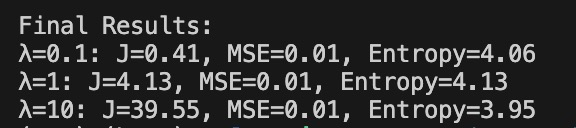
\includegraphics[width=0.8\textwidth]{result.png} 
        \caption{result}  
    \end{figure}
    我们把重构和重构前的数据可视化一下:
    \begin{figure}[ht]
        \centering
        \label{compression}
        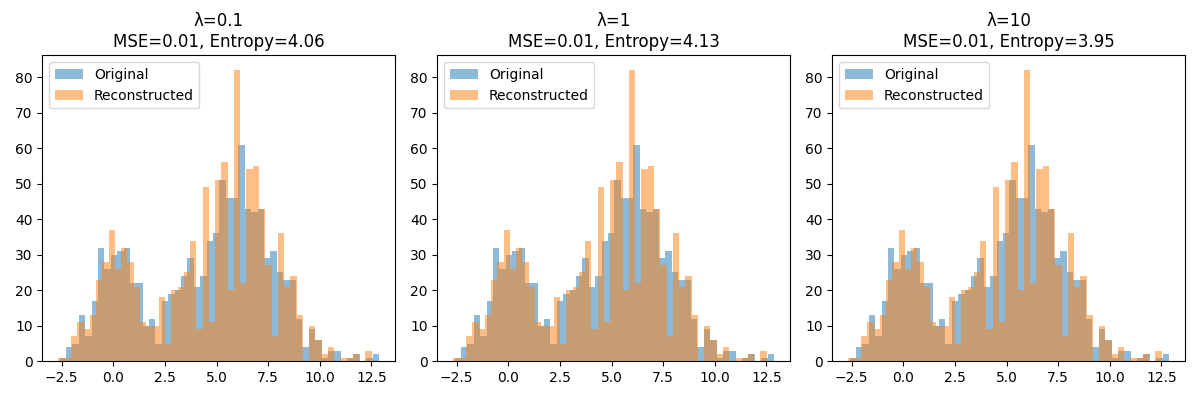
\includegraphics[width=0.8\textwidth]{compression_results.png} 
        \caption{compression}  
    \end{figure}
    可以看出,MSE都比较小,$\lambda$对于码率的限制确实是有效果的。
\end{enumerate}

\end{document}